\documentclass[a4paper,11pt,twoside]{article}
\usepackage[T1]{fontenc}
\usepackage[utf8]{inputenc}
\usepackage[swedish]{babel}

\usepackage[margin=1in]{geometry}
\usepackage{amsfonts, amsmath, amssymb}
\usepackage[none]{hyphenat}
\usepackage{fancyhdr}
\usepackage[nottoc, notlot, notlof]{tocbibind}
\usepackage{mathtools}

\usepackage{graphicx}

\usepackage{url}
%%  Defines the command \url{} that can be used to typeset url:s
%%  in text

\usepackage[parfill]{parskip}

\setcounter{tocdepth}{4}
\setcounter{secnumdepth}{4}


\newcommand*{\pd}[2]{\ensuremath{\dfrac{\partial #1}{\partial #2}}}
\newcommand*{\inpd}[2]{\ensuremath{\frac{\partial #1}{\partial #2}}}
\DeclarePairedDelimiter\floor{\lfloor}{\rfloor}



\title{Matematik och Konvolutionella Neurala Nätverk för dataseende}
\title{eller}
\title{Objektdetektering och Ansiktsigenkänning med Konvolutionella Neurala Nätverk}
\author{Nikita Zozoulenko}
\date{\today}

\begin{document}



\begin{titlepage}
\maketitle
\end{titlepage}


%start abstract
\Large{\textbf{Abstract}}\\\\
Convolutional Neural Networks have ...
\newpage
%end abstract

\tableofcontents

\section{Introduktion}

\subsection{Bakgrund}
25 sidor av min rapport är bakgrund ?????

nej men seriöst vet inte  vad jag ska skriva här, råd och förslag välkomnas starkt
\subsection{Syfte}
Syftet med arbetet är att redogöra för den underliggande matematiken bakom den matematiska modellen av klassiska neurala nätverk och konvolutionella neurala nätverk, samt visa exempel på praktiska tillämpningar.
\subsection{Frågeställning}
Vad är ett artificiellt neuralt nätverk?
Vad är ett Konvolutionellt Neuralt Nätverk?
Hur härleds framåt- och bakåtpropageringen i feed-forward neurala nätverk och konvolutionella neurala nätverk?
Hur kan modellen tillämpas för att implementera sifferavläsning,ansiktsigenkänning och objektdetektion i bilder?


\newpage
\section{Metod}

Majoriteten av tiden gick åt till att... standford, vetenskapliga artiklar batch normalization någonting et al. 2015.... implementera skiten och dubbelkolla med derivatans definition

\newpage
\section{Notation och Tensorer}
I denna rapport används notation för bland annat vektorer, matriser och tensorer av högre grad. En tensor av grad 1 är en vektor $x \in \mathbb{R}^H$ och är en radvektor med $H$ element. Det kan dessutom ses som en endimensionell array. Matriser $M$ är tensorer av grad 2 sådana att $M \in \mathbb{R}^{H \times W}$ och kan ses som en vektor av vektorer eller en tvådimensionell array. Tensorer kan alltså ses som en generalisering av vektor- och matrisbegräppen. En tensor $X \in \mathbb{R}^{R \times C \times H \times W}$ av grad 4 indexeras med en fyr-tupel $(r,c,h,w)$ där $0 \leq r < R$, $0 \leq c < C$, $0 \leq h < H$ och $0 \leq w < W$. 

%Om $R \times C \times H \times W$ och $(r,c,h,w)$ representerar dimensionerna respektive index för lager $l$ represneterar $R \times C' \times H' \times W'$ och $(r,c',h',w')$ dimensionerna respektive index för nästinkommande lager.

Om $X$ är en matris definieras funktionen $f(X)$ genom att elementvis applicera $f$ på alla matrisens element:
\begin{align}
	f(X) = 
	& \begin{bmatrix}
	f(X_{0,0}) & f(X_{0,1}) & \cdots & f(X_{0,i}) \\
	f(X_{1,0}) & f(X_{1,1}) & \cdots & f(X_{1,i}) \\
	\vdots     & \vdots     & \ddots & \vdots     \\
	f(X_{j,0}) & f(X_{j,1}) & \cdots & f(X_{j,i}) \\
	\end{bmatrix} \\
\pd{f(X)}{X} = 
	& \begin{bmatrix}
	\pd{f(X_{0,0})}{X_{0,0}} & \pd{f(X_{0,1})}{X_{0,1}} & \cdots & \pd{f(X_{0,i})}{X_{0,i}} \\
	\pd{f(X_{1,0})}{X_{1,0}} & \pd{f(X_{1,1})}{X_{1,1}} & \cdots & \pd{f(X_{1,i})}{X_{1,i}} \\
	\vdots                   & \vdots                   & \ddots & \vdots     \\
	\pd{f(X_{j,0})}{X_{j,0}} & \pd{f(X_{j,1})}{X_{j,1}} & \cdots & \pd{f(X_{j,i})}{X_{j,i}} \\
	\end{bmatrix}
\end{align}

Detta kan generaliseras för en tensor av grad n:
\begin{equation}\label{f(x)}
	\begin{bmatrix} f(X) \end{bmatrix}_{i_0, i_1, \cdots, i_{n-1}}
	= f(X_{i_0, i_1, \cdots, i_{n-1}})
\end{equation}
\begin{equation}\label{f'(x)}
	\begin{bmatrix}
	\pd{f(X)}{X}
	\end{bmatrix}_{i_0, i_1, \cdots, i_{n-1}}
	=
	\pd{f(X_{i_0, i_1, \cdots, i_{n-1}})}{X_{i_0, i_1, \cdots, i_{n-1}}}
\end{equation}

Hadamardprodukten betäcknas med $\odot$ och verkar på två tensorer $A$ och $B$ av samma storlek och producerar en tensor $C$ med samma storlek.\cite{cs231n} Elementen i tensorerna multipliceras elementvist : 
\begin{equation}
	C_{i_0, i_1, \cdots, i_{n-1}} = A_{i_0, i_1, \cdots, i_{n-1}} \odot B_{i_0, i_1, \cdots, i_{n-1}}
\end{equation}

En tensor av grad n kan ses som en tensor av grad 1 vars element är tensorer av grad n-1. Exempelvis är en vektor en vektor av skalärer och en matris en vektor av vektorer. Funktionen $vec()$ gör om en tensor av grad n till en vektor genom att rekursivt använda den sistnämnda egenskapen av tensorer. \cite{convmath}

\section{Resultat}
\subsection{Feed-forward Neurala Nätverk}
Ett artificellt neuralt nätverk består av ett antal lager neuroner. De är uppbyggda rekursivt så att resultatet av ett lager är inmatningen till nästintilliggande lager. Nervsignalen propageras framåt tills den når det sista lagret. Hur nervceller från ett lager är kopplade till det föregående lagret varierar med vilken typ av neuralt nätverk man väljer. \cite{cs231n}

Den mest grundläggande modellen har flera namn, bland annat:  \textit{Multilayer Perceptrons} \textit{Fully Connected Cascade (FCC)}, \textit{Feed-forward Neural Network} och \textit{Densly Connected (Dense)}. Den består av ett flertal lager av neuroner. Varje neuron i ett lager är kopplade till alla neuroner i nästintillföljande lager. Nervsignalen framåtpropageras beroende på hur stark kopplingen mellan två neuroner är. Ett neurons värde kallas för dess aktivering. \eqref{f(x)}. \cite{cs231n}

% Utöver den vanliga nervsignalsöverföringen appliceras dessutom en aktiveringsfunktion $f(x)$ på samtliga lager elementvis på varje neuron enligt ekvation 

\begin{figure}[h]\label{figFCC}
	\centering
  		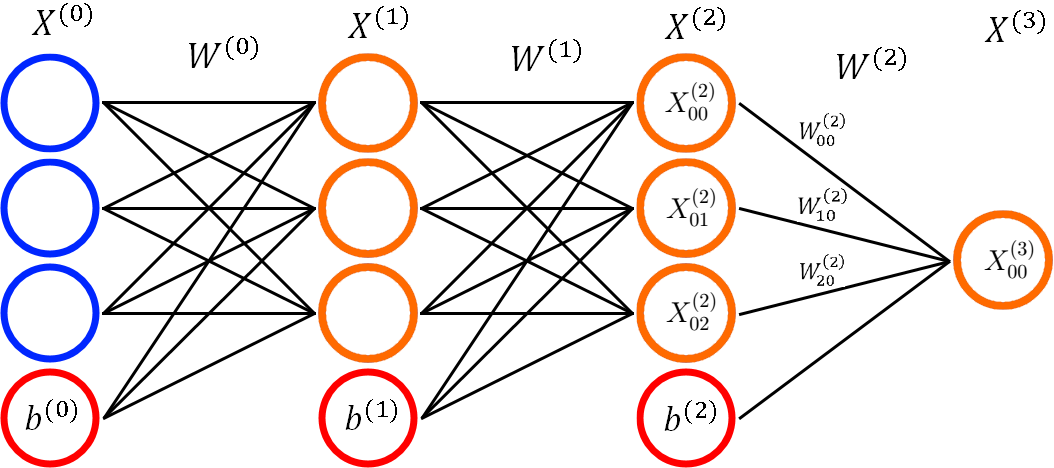
\includegraphics[scale=0.4]{FCC.png}
  	\caption{Ett exempel på ett enkelt feed-forward neuralt nätverk. Inputneuronerna är blåmarkerade medan resterande neuroner är orangea. Röda neuroner är så kallade ”bias-neuroner” som är konstanta oberoende på inputdatan. Svarta linjer symboliserar vikterna och deras styrka mellan två neuroner.}
\end{figure}

\subsubsection{Framåtprogagering}
\textit{Forward propagation} eller framåtpropagation är processen av att från sina inputneuroner propagera framåt nervsignalen i nätverket tills man når outputlagret. \cite{cs231n} \cite{wikiStanford}

Nätverket kan framställas genom att representera neuronerna och deras kopplingar m.h.a matriser. Låt $X_{ri}^{(l)}$ benämna neuron nummer $i$ i lager $l$ i träningsexempel $r$. $W_{ba}^{(l)}$ blir vikten eller styrkan på kopplingen mellan neuron $X_{ra}^{(l)}$ och $X_{rb}^{(l+1)}$. Låt $b^{(l)}$ vara ett konstant neuron som är kopplad till alla neuron i lager $l+1$.  \cite{cs231n} \cite{wikiStanford}

För att beräkna aktiveringen av ett neuron i lager $l+1$ multipliceras varje neurons värde i lager $l$ med deras korresponderande vikt i viktmatrisen $W^{(l)}$. Resultaten och lagrets konstanta neuron $b^{(l)}$ summeras och summan matas in i en aktiveringsfunktion $f(x)$. Funktionsvärdet blir aktiveringen i det nya neuronet. Exempelvis kan signalöverföringen mellan lager 2 och 3 i figur 1 beskrivas matematiskt genom: \cite{cs231n} \cite{wikiStanford}

%Output av nätverket kallas för $\hat{y}$ och är värdet av det sista lagret neuroner. 

\begin{equation}
\begin{split}
X_{00}^{(3)} & = f(X_{00}^{(2)}W_{00}^{(2)} + X_{01}^{(2)}W_{10}^{(2)} + X_{02}^{(2)}W_{20}^{(2)} + b^{(2)}) \\
\end{split}
\end{equation}
%& = f(X^{(2)}W^{(2)} +b^{(2)})

Där $X^{(3)} \in \mathbb{R}^{1 \times 1}$, $X^{(2)} \in \mathbb{R}^{1 \times 3}$, $W^{(2)} \in \mathbb{R}^{3 \times 1}$ och $b^{(2)} \in \mathbb{R}^{1}$.

Neuronmatriserna och viktmatriserna är definierade på ett sådant sätt att framåtpropegationen mellan lager $l$ och $l+1$ kan beräknas med en matrismultiplikation och kan därför beräknas rekursivt från inputneuronerna: \cite{cs231n} \cite{wikiStanford}

\begin{equation}\label{feed-forward}
X^{(l+1)} = f(X^{(l)}W^{(l)} +b^{(l)})
\end{equation}

Vanliga aktiveringsfunktioner för neurala nätverk är \textit{Rectified Linear Units ($ReLU$)}, \textit{sigmoid ($\sigma$)} och \textit{tangens hyperbolicus ($tanh$)}. Funktionerna måste vara deriverbara för att nätverket ska kunna tränas genom processen som kallas för bakåtpropagering. Genom att använda olinjära funktioner kan nätverket lära sig olinjära samband. Definitionerna av funktionerna ges av: \cite{cs231n} 

\begin{figure}[h]\label{aktiveringsfunktion}
	\centering
  		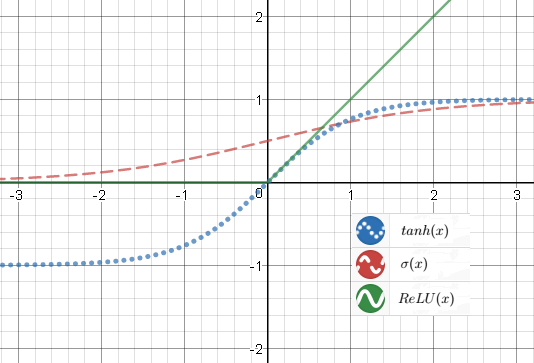
\includegraphics[scale=0.8]{activationfunction.png}
  	\caption{Grafen av aktiveringsfunktionerna $ReLU$, $\sigma$ och $tanh$.}
\end{figure}

\begin{equation}
ReLU(x) = \begin{cases} 
			0 & \mbox{om } x < 0 \\ 
			x & \mbox{om } x \geq 0 
		\end{cases}
\end{equation}

\begin{equation}
\sigma(x) = \frac{1}{1+e^{-x}}
\end{equation}

\begin{equation}
tanh(x) = \frac{e^x-e^{-x}}{e^x+e^{-x}}
\end{equation}

För att derivera $ReLU$ deriveras varje enskilda fall:

\begin{equation}
\pd{(ReLU(x))}{x} = \begin{cases} 
			0 & \mbox{om } x < 0 \\ 
			1 & \mbox{om } x \geq 0 
		\end{cases} \quad
\end{equation}

Notera att:

\begin{equation}
\lim_{x\to 0^+} ReLU(x) = 1
\end{equation}

\begin{equation}
\lim_{x\to 0^-} ReLU(x) = 0
\end{equation}

Trots att derivatan av ReLU inte är definierad i punkten $x = 0$ sätts $\inpd{(ReLU(x))}{x}|_{\substack{x=0}}$ vara lika med $0$ eller $1$ utan att några problem tillkommer. \cite{cs231n} 


Kvotregeln tillämpas för att härleda derivatan av $\sigma$ och $tanh$:

\begin{equation}
\begin{split}
\pd{\sigma(x)}{x} 	& = \frac{e^{-x}}{(1+e^{-x})^2} \\
					& = \frac{1}{1+e^{-x}}(\frac{1+e^{-x}}{1+e^{-x}}-\frac{1}{1+e^{-x}})\\
			 		& = \sigma(x)(1-\sigma(x))
\end{split}
\end{equation}

\begin{equation}
\begin{split}
\pd{(tanh(x))}{x} 	& = \frac{(e^x+e^{-x})(e^x+e^{-x})-(e^x-e^{-x})(e^x-e^{-x})}{(e^x+e^{-x})^2} \\
					& = 1 - \frac{(e^x-e^{-x})^2}{(e^x+e^{-x})^2} \\
			 		& = 1 - {tanh}^2(x)
\end{split}
\end{equation}



\subsubsection{Bakåtpropagation}
Givet ett inputvärde för X skapas ett närmevärde $\hat{y}$ som ska vara så nära det sanna värdet för y som möjligt. När man först initialiserar modellen kommer vikterna $W^{(l)}$ vara slumpade och nätverkets prognos kommer inte efterlikna det sökta värdet. Med hjälp av \textit{gradient descent} kan man iterativt träna modellen så det slutgiltiga värdet kommer så nära y som möjligt. Detta görs genom att definiera en multivariat kostnadsfunktion $L(W, b; X,y)$ av variablerna $W^{(0)}$, $W^{(1)}$, ..., $W^{(l)}$, $b^{(0)}$, $b^{(1)}$, ..., $b^{(l)}$ med avseende på ett träningsexempel $(X, y)$. Funktionen är ett mått på prognosen $\hat{y}$ kvalitet. Man definierar $L$ på ett sådant sätt att ju liten värdemängd av $L$, desto högre kvalitet består $\hat{y}$ av. Ett sätt att definiera $L$ är exempelvis med en så kallad \textit{L2 kostnadsfunktion}: \cite{cs231n} \cite{wikiStanford}
\begin{equation}
\begin{split}
L(W,b) 	& = {||\hat{y}-y_r||}^2 \\
		& = {||f(f(f(XW^{(0)} +b^{(0)})W^{(1)} +b^{(1)})W^{(2)} +b^{(2)}) - y||}^2
\end{split}
\end{equation}
Gradienten $\nabla L(\theta)$ är en vektor av partiella derivator med avseende på funktionen $L$ variabler $W^{(0)}$, $W^{(1)}$, ..., $W^{(l)}$, $b^{(0)}$, $b^{(1)}$, ..., $b^{(l)}$ som definieras genom: \cite{gradient} \cite{convmath} 
\begin{equation}
\nabla L(\theta) : \mathbb{R}^n \to \mathbb{R}^n
\end{equation}
\begin{equation}
\nabla L(\theta) = 
	\begin{pmatrix} 
		\pd{L(\theta)}{\theta^{(0)}} & 
		\pd{L(\theta)}{\theta^{(1)}} &
		\cdots &
		\pd{L(\theta)}{\theta^{(n-1)}}
		
		\end{pmatrix}
\end{equation}

Gradienten $\nabla L(\theta)$ visar riktningen vari värdemängdsökningen är som störst. Genom att ändra vikterna $\theta$ värde proportionellt med avseende på den negativa gradienten $-\nabla L(\theta)$ kan man iterativt modifiera $\theta$ tills man når funktionens minimum. Den mest grundläggande algoritmen för \textit{gradient descent} kallas för \textit{Stochastic Gradiant Descent (SGD)} och använder hyperparametern $\alpha$ för att beteckna träningshastigheten: \cite{gradient} \cite{convmath} \cite{wikiStanford}

\begin{equation}
\pd{L(\theta)}{\theta^{(l)}} = \nabla_{\theta^{(l)}} L(\theta)
\end{equation}
\begin{equation}
\theta^{(l)} \to \theta^{(l)} - \alpha \pd{L(\theta)}{\theta^{(l)}}
\end{equation}
\begin{figure}[h]\label{figSGD}
	\centering
  		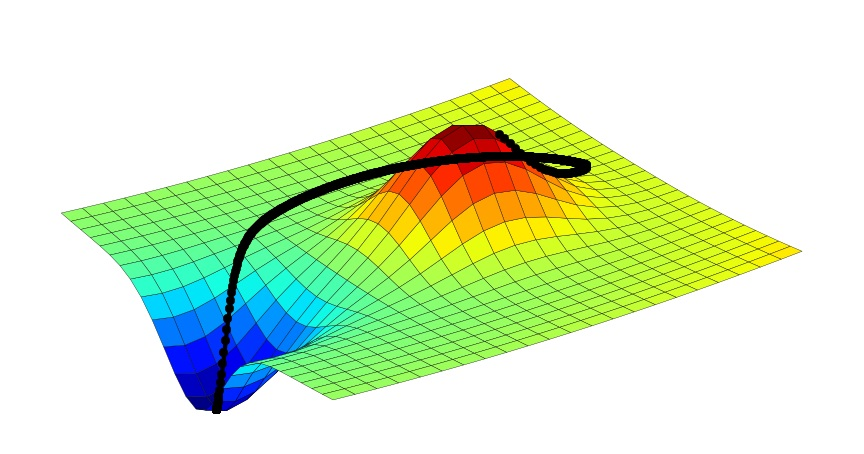
\includegraphics[scale=0.5]{SGD.png}
  	\caption{En illustration av gradient descent på en funktion med två variabler \cite{figSGD}}
\end{figure}

De partiella derivatorna kan approximeras med hjälp av framåt, bakåt eller central differenskvot för partiella derivator: \cite{wikiStanford} \cite{gradient}

\begin{equation}
\pd{L(\theta)}{\theta^{(i)}} = \frac{L(\theta^{(0)},...,\theta^{(i)} + h, ..., \theta^{(n-1)})-L(\theta)}{h}
\end{equation}

Detta skulle inte skapa några problem för det lilla neurala nätverket i figur 1 med 24 parametrar, men i själva verket har djupa neurala nätverk miljontals av parametrar som skulle behöva en enorm datorkraft. Istället kan man tillämpa regler för matriskalkyl och kedjeregeln för att effektivt beräkna de partiella derivatorna. Genom att använda ett kedjeliknande argument kan derivatorna uttryckas som: \cite{cs231n} \cite{convmath}

\begin{equation}
\pd{L(\theta)}{(vec(W^{(l)})^T)} = \pd{L(\theta)}{(vec(X^{(l+1)})^T)} \pd{(vec(X^{(l+1)}))}{(vec(W^{(l)})^T)}
\end{equation}

\begin{equation}
\pd{L(\theta)}{(vec(b^{(l)})^T)} = \pd{L(\theta)}{(vec(X^{(l+1)})^T)} \pd{(vec(X^{(l+1)}))}{(vec(b^{(l)})^T)}
\end{equation}

Där

\begin{equation}
\pd{L(\theta)}{(vec(X^{(l)})^T)} = \pd{L(\theta)}{(vec(X^{(l+1)})^T)} \pd{(vec(X^{(l+1)}))}{(vec(X^{(l)})^T)}
\end{equation}

För att $\inpd{X^{(l+1)}}{X^{(l)}}$, $\inpd{X^{(l+1)}}{W^{(l)}}$, $\inpd{X^{(l+1)}}{b^{(l)}}$ och derivatan av $L$ med avseende på det sista lagret är möjliga att beräknas algebraiskt är det därför möjligt att rekursivt beräkna gradienten genom att bakåtpropagera i nätverket från outputlagret. Värdena från det nästkommande lagret används för att beräkna värdena för det föregående lagret. \cite{convmath}

Betrakta ekvation (\ref{feed-forward}). Om $L$ är en L2 kostandsfunktion beräknas de partiella derivatorna enligt:  \cite{cs231n} \cite{convmath} 

\begin{equation}
\begin{split}
\pd{L(\theta)}{\hat{y}} 
				& = 2 ||\hat{y}-y|| \\
\end{split}
\end{equation}

I följande ekvationer utnyttjas $\inpd{AB}{B} = A^T$ och $\inpd{AB}{A} = B^T$ tillsammans med kedjeregeln.
\begin{equation}
\begin{split}
\pd{X^{(l+1)}}{X^{(l)}} 
				& = \pd{f(X^{(l)}W^{(l)} +b^{(l)})}{X^{(l)}}  \\
				& = f'(X^{(l)}W^{(l)}+b^{(l)})W^{(l)^T}
\end{split}
\end{equation}

\begin{equation}
\begin{split}
\pd{X^{(l+1)}}{W^{(l)}} 
				& = \pd{f(X^{(l)}W^{(l)} +b^{(l)})}{X^{(l)}}  \\
				& = X^{(l)^T}f'(X^{(l)}W^{(l)}+b^{(l)})
\end{split}
\end{equation}

\begin{equation}
\begin{split}
\pd{X^{(l+1)}}{b^{(l)}} 
				& = \pd{f(X^{(l)}W^{(l)} +b^{(l)})}{X^{(l)}}  \\
				& = f'(X^{(l)}W^{(l)}+b^{(l)})
\end{split}
\end{equation}

Här kan man se varför aktiveringsfunktionerna behöver vara deriverbara.

I praktiken beräknas de partiella derivatorna med hjälp av en rekursiv formel. Låt: \cite{cs231n} \cite{wikiStanford} \cite{convmath}
\begin{equation}
\delta^{(l)} = \pd{L(\theta)}{X^{(l)}}
\end{equation}
Det (också kallat delta-felet) är den bakåtpropagerade nervsignalen upp till lager $l$. Om $l_{sista}$ är det sista lagret definieras delta-felen och gradienten enligt följande formler för en L2 kostandsfunktion: \cite{cs231n} \cite{wikiStanford} \cite{convmath}

\begin{equation}
\delta^{(l_{sista})} = 2 ||\hat{y}-y||
\end{equation}

\begin{equation}
\begin{split}
\delta^{(l)} 
	& = \pd{L(\theta)}{X^{(l)}} \\
	& = \pd{L(\theta)}{X^{(l+1)}} \pd{X^{(l+1)}}{X^{(l)}}\\
	& = \left( \delta^{(l+1)} \odot f'(X^{(l)}W^{(l)}+b^{(l)}) \right) W^{(l+1)^T}\\
\end{split}
\end{equation}

\begin{equation}
\begin{split}
\pd{L(\theta)}{W^{(l)}}
	& = \pd{L(\theta)}{X^{(l+1)}} \pd{X^{(l+1)}}{W^{(l)}}\\
	& = X^{(l)^T} \left( \delta^{(l+1)} \odot f'(X^{(l)} W^{(l)}+b^{(l)}) \right) \\
\end{split}
\end{equation}

\begin{equation}
\begin{split}
\pd{L(\theta)}{b^{(l)}}
	& = \pd{L(\theta)}{X^{(l+1)}} \pd{X^{(l+1)}}{b^{(l)}}\\
	& =  \delta^{(l+1)} \odot f'(X^{(l)} W^{(l)}+b^{(l)})  \\
\end{split}
\end{equation}

Två implementationer av ett feedforward neuralt nätverk kan hittas på github i python och C++: \url{https://github.com/nikitazozoulenko}

\subsection{Konvolutionella Neuala Netvärk}
När människor vill identifiera någonting i en bild så letar vi efter vissa karakteristiska drag objektet har. En hund består exempelvis av en kropp, ett huvud och fyra ben. Kroppsdelarna består sedan själva av grundläggande geometriska former som i sig självt är kombinationer av kanter och linjer. Dessutom har hundar en viss textur, det som vi kännetecknar som något pälsliknande. Dessa karakteristiska drag är lokala inom bilden och kan extraheras av att endast se på en liten del av bilden i taget.Det är just detta som är principen bakom \textit{Konvolutionella Neurala Nätverk (CNN)}: Genom så kallade \textit{konvolutioner} kunna extrahera dessa karakteristiska drag. Nätverket lär sig ett antal filter väldigt små filter som den applicerar på en delmängd av bilden genom att filtret sammanrullar över hela bilden. Värdet av filtret över en delmängd av bilden blir aktiveringen av ett neuron i nästa lager.  \cite{cs231n}

\begin{figure}[h]\label{figkatter}
	\centering
  		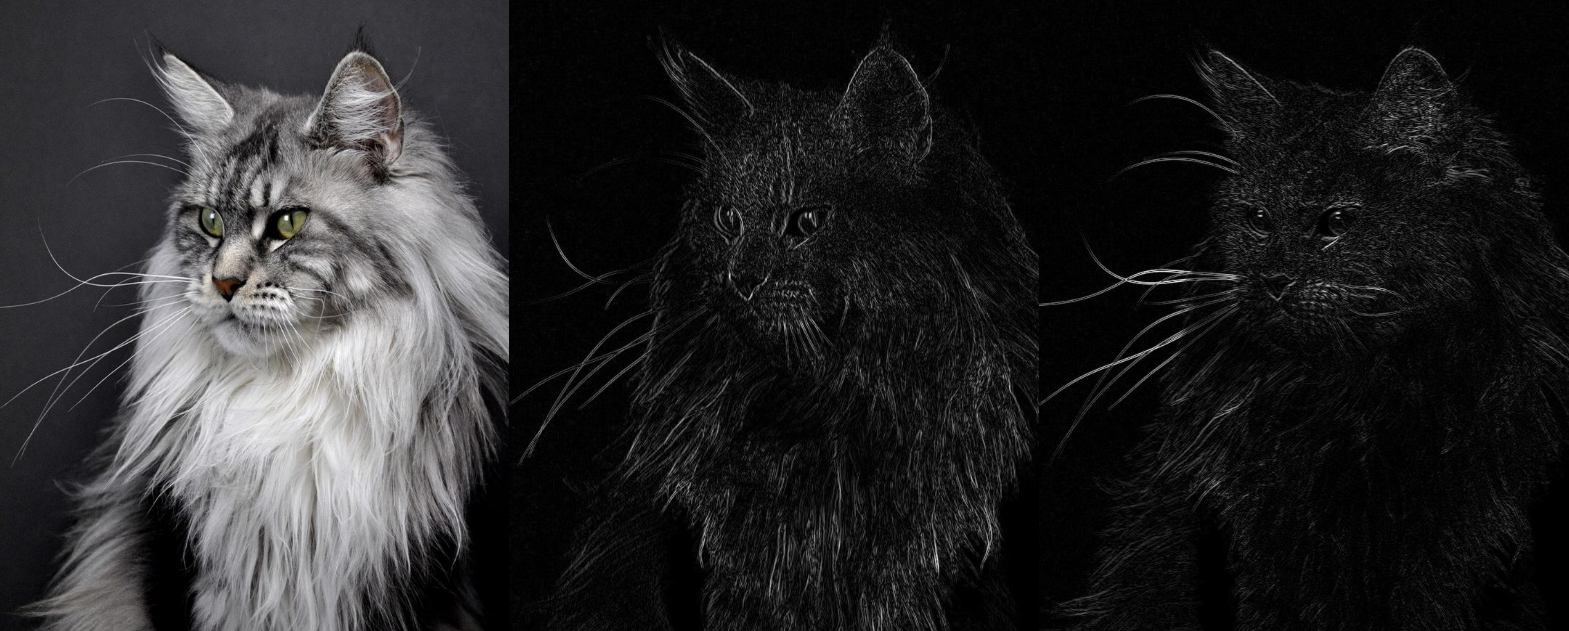
\includegraphics[scale=0.33]{katter.png}
  	\caption{Resultatet av ett en kärna för horizontell och vertikal kantdetektering har sammanrullat över en bild av en katt.}
\end{figure}

Till skillnad från \textit{FCC} är neuronerna i ett \textit{CNN} bara kopplade till närliggande neuroner i det föregående lagret. På detta sätt kan nätverket lära sig fler hög-nivåspecialartiklar ju djupare i nätverket signalen går. Exempelvis kan det hända att det första lagret identifiera kanter och linjer medan de senare lagren lagren känner igen olika former och till sist känna igen ansikten eller object i sista lagert. \cite{cs231n}

Modellen, precis som ett \textit{feed-forward nätverket}, består av ett flertal lager neuroner sådant att resultatet av ett lager matas in till nästkommande lager. För ett \textit{FCC} användes en matris för att representera neuronerna. I ett \textit{CNN} är en tensor $X^{(l)} \in \mathbb{R}^{R \times C  \times H \times W}$ av grad 4 aktiveringen vid lager $l$. Aktiveringen brukar illustreras som en tredimensionell volym där $W$, $H$ och $C$ är bredden, höjden respektive djupet. En $H \times W$ skiva av volymen kallas för en \textit{feature map} eller en \textit{kanal}. Antalet kanaler benämns med $C$. $R$ står för hopstorlek då man bearbetar R exempel i taget i en så kallad mini-hop. Vid varje lager finns dessutom vikter $W^{(l)}$  som beror på vad för slags lager det är. $W^{(l)}$ kan vara tom med inga vikter när lager inte bidrar till någon inlärning. \cite{cs231n} \cite{convmath}

\begin{figure}[h]\label{figboatcnn}
	\centering
  		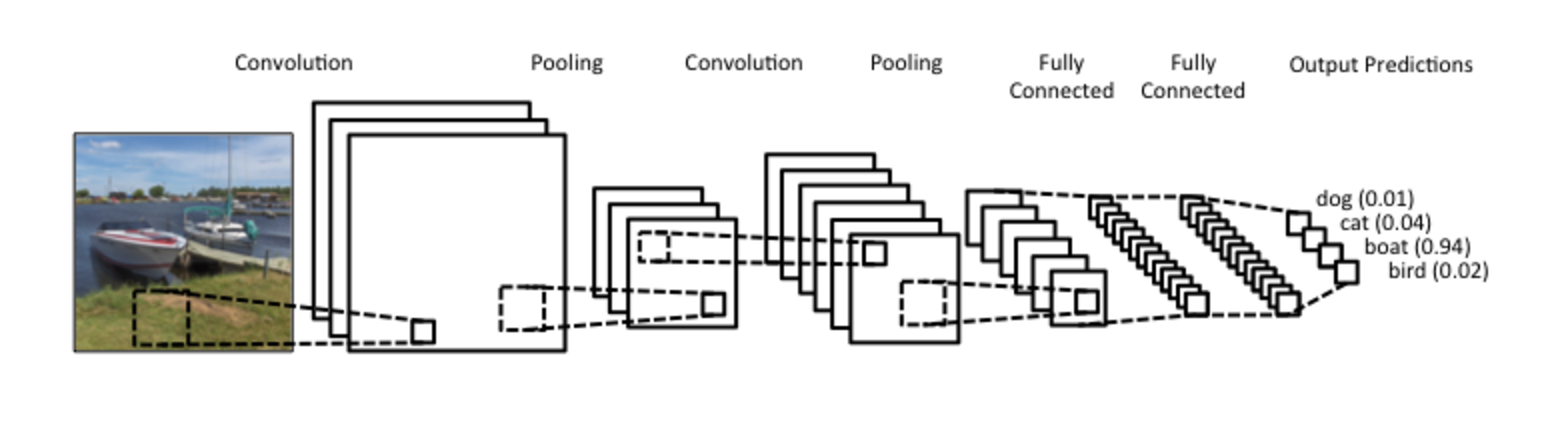
\includegraphics[scale=0.6]{boatcnn.png}
  	\caption{En illustration av ett konvolutionellt neuralt nätverk. \cite{figboatcnn}}
\end{figure}

För att en konvolution är en lokal operator används CNNs för data som innehåller lokalt sammanhängande samband, exempelvis bilder eller ljud. Om det är en bild som bearbetas har det första lagrets aktivering $C = 3$ kanaler, en för varje RGB-kanal, och en bredd och höjd lika med bildens bredd och höjd i pixlar. \cite{cs231n} \cite{convmath}

\subsubsection{Konvolutionslagret framåtpropagering}
Ett konvolutionslager består av ett antal vikter kallade \textit{kärnor (kernels)} eller \textit{masker (masks)}, representerade av en tensor av grad fyra, $W^{(l)} \in \mathbb{R}^{C' \times C  \times k_h \times k_W}$ för lager $l$. \cite{cs231n} \cite{convmath}

När masken är över en godtycklig del av volymen multipliceras varje värde i delmängden av $W^{(l)}$ elementvis med respektive värde i masken vid samma position och summeras (se figur 6). Summan blir aktiveringen av ett neuron i nästa lager. Konvolutionsoperatorn betecknas med $*$. \cite{cs231n} \cite{convmath}

\begin{figure}[h]\label{figkonv}
	\centering
  		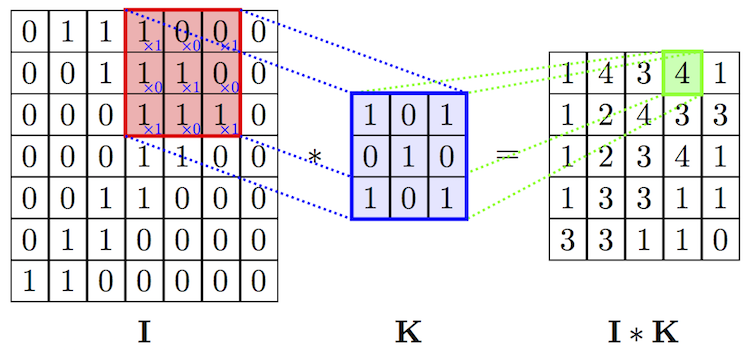
\includegraphics[scale=2.1]{convolution.png}
  	\caption{En kärna med storlek $3 \times 3$ sammanrullar över ett område med dimensioner $6 \times 6$ och bildar en aktivering med dimensionerna $4 \times 4$. \cite{figkonv}}
\end{figure}

En feature map i lager $l+1$ är resultatet av att en kärna med dimensioner $1 \times \times C  \times k_h \times k_W$ har sammanrullat över aktiveringen av det föregående lagret. $C'$ är antalet kärnor och blir dessutom antalet feature maps nästa lager har. \cite{cs231n} \cite{convmath}

Kärnorna har två ytterligare egenskaper: ett kliv $s$ och så kallad \textit{zero-padding} $p$. $s$ är hur stort kliv man tar efter varje gång filtret blir applicerat på tensorn. Man ökar tensorns höjd och bredd med $2p$ genom att fylla på med nollor vid tensors ändor (se figur 7). På grund av att aktiveringens höjd och bredd avtar ju djupare i nätverket de befinner sig på används zero-padding för att kontrollera storleken av tensorn. \cite{cs231n} \cite{convmath} \cite{convarithmetic}

Låt $W^{(l)} \in \mathbb{R}^{C' \times C  \times k_h \times k_W}$, $X^{(l)} \in \mathbb{R}^{R \times C  \times (H+2p) \times (W+2p)}$ och $X^{(l+1)} \in \mathbb{R}^{R \times C'  \times H' \times W'}$. Dimensionerna vid lager $l+1$ beskrivs av: \cite{cs231n} \cite{convmath} \cite{convarithmetic}
\begin{equation}
W' = \frac{W-k_W+2p}{s} +1
\end{equation}
\begin{equation}
H' = \frac{H-k_H+2p}{s} +1
\end{equation}

\begin{figure}[h]\label{figzeropad}
	\centering
  		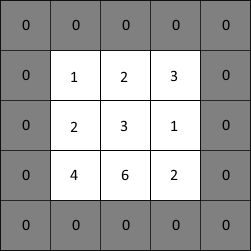
\includegraphics[scale=0.7]{zeropadding.png}
  	\caption{Ett område med dimensioner $3 \times 3$ zero-paddas med $p=1$ och resulterande område får dimensioner $5 \times 5$.}
\end{figure}

Då beskrivs en konvolution algebraiskt genom: \cite{cs231n} \cite{convmath}
\begin{equation}
w = sw'
\end{equation}
\begin{equation}
h = sh'
\end{equation}
\begin{equation}\label{konvolution}
\begin{split}
	\begin{bmatrix} X^{(l+1)} \end{bmatrix}_{r, c', h', w'}	
		& = X^{(l)}_{r, c', h', w'} *W^{(l)}_{c'} \\
		& = \sum^{C-1}_{c=0} \sum^{k_H-1}_{j=0} \sum^{k_W-1}_{i=0} X^{(l)}_{r, c, h'+j, w'+i}W^{(l)}_{c', c, j, i}
\end{split}
\end{equation}

Index på termen som ska sammanrullas i konvolutionen symboliserar vilka dimensioner som ska summeras. Exempelvis visar $W^{(l)}_{c'}$ att dimensionerna $C$, $H$ och $W$ (alla kanaler) ska summeras medan  $W^{(l)}_{c', c}$ visar att endast $H$ och $W$ (en kanal) ska summeras.

I praktiken brukar konvolutioner implementeras med hjälp av funktionerna $row2im$ och $im2row$ vilka lämnas till läsaren att läsa på om om han eller hon vill optimera hur snabbt konvolutionen beräknas. \cite{cs231n} \cite{convmath} \cite{convarithmetic}

\subsubsection{Konvolutionslagret bakåtpropagering}
Bakåtpropegeringen förstås bäst genom att algebraiskt härleda den. 

Bakåtpropageringen av det rekursiva delta-felet $\inpd{L(W)}{X^{(l+1)}_{r,c',h',w'}}$ räkas ut med hjälp av kedjeregeln. Derivatan kan inte endast delas upp i $\inpd{L(W)}{X^{(l+1)}_{r,c',h',w'}}$ och $\inpd{X^{(l+1)}_{r,c',h',w'}}{X^{(l)}_{r,c,h,w}}$, utan alla derivator måste summeras på grund av att det är mer än ett neuron som är ansvarig för framåtpropageringen. $X^{(l+1)}_{r,c',h',w'}$ byts sedan ut mot dess definition enligt ekvation \eqref{konvolution}. \cite{convmath} \cite{webconv1} \cite{webconv2} \cite{webconv3}
\begin{equation}\label{konvolutionbackprop}
\begin{split}
	\delta^{(l)}_{r,c,h,w}
		& = \pd{L(W)}{X^{(l)}_{r,c,h,w}} \\
		& = \sum^{C'-1}_{c'=0} \sum^{H'-1}_{h'=0} \sum^{W'-1}_{w'=0} \pd{L(W)}{X^{(l+1)}_{r,c',h',w'}} \pd{X^{(l+1)}_{r,c',h',w'}}{X^{(l)}_{r,c,h,w}} \\
		& = \sum^{C'-1}_{c'=0} \sum^{H'-1}_{h'=0} \sum^{W'-1}_{w'=0} \delta^{(l+1)}_{r,c',h',w'} \pd{\sum^{C-1}_{c=0} \sum^{k_H-1}_{j=0} \sum^{k_W-1}_{i=0} X^{(l)}_{r, c, h'+j, w'+i}W^{(l+1)}_{c', c, j, i}}{X^{(l)}_{r,c,h,w}}
\end{split}
\end{equation}
Varje produkt i den innersta summan kommer att vara like med noll förutom om $X^{(l)}_{r, c, h'+j, w'+i} = X^{(l)}_{r,c,h,w}$. Förljaktligen insätter man $h'+j = h$ och $h'+j = h$. Summorna och derivatan förkortas: \cite{webconv1} \cite{webconv2} \cite{webconv3}
\begin{multline}
\sum^{C'-1}_{c'} \sum^{H'-1}_{h'=0} \sum^{W'-1}_{w'=0} \delta^{(l+1)}_{r,c',h',w'} \pd{\sum^{C-1}_{c=0} \sum^{k_H-1}_{j=0} \sum^{k_W-1}_{i=0} X^{(l)}_{r, c, h'+j, w'+i}W^{(l+1)}_{c', c, j, i}}{X^{(l)}_{r,c,h,w}} \\
	\begin{split}
	 = \sum^{C'-1}_{c'=0} \sum^{H'-1}_{h'=0} \sum^{W'-1}_{w'=0} \delta^{(l+1)}_{r,c',h',w'} W^{(l+1)}_{c', c, j, i} \\
	 = \sum^{C'-1}_{c'=0} \sum^{H'-1}_{h'=0} \sum^{W'-1}_{w'=0} W^{(l+1)}_{c', c, (h-h'), (w-w')}  \delta^{(l+1)}_{r,c',h',w'}   \\
	 \end{split}
\end{multline}
Vilket man kan se är en summa av konvolutioner där en viss feature map av delta-felet sammanrullar över alla kärnor på en viss feature map med vikter som är roterade $180^\circ$. För att en konvolution ska kunna ske måste den roterade vikten zero-paddas på grund av att det glidande fönstret måste vara som mest lika stor som tensorn den sammanrullar över. Låt rotationen betäcknas med funktionen $rot()$. \cite{webconv1} \cite{webconv2} \cite{webconv3}
\begin{equation}
\delta^{(l)}_{r,c,h,w} = \sum^{C'-1}_{c'=0} rot(W^{(l+1)}_{c',c,h,w}) * \delta^{(l+1)}_{r,c'}
\end{equation}
En sundshetskontroll visar att detta är intuitivt då alla feature maps i $X^{(l)}$ används för att skapa en enstaka feature map i $X^{(l+1)}$. Det är därför man summerar över alla kärnor och endast konvolverar i en feature map i taget och summerar alltihop.

Den partiella derivatan av kostandsfunktionen med avseende på vikterna hittas på ett liknande sätt: \cite{webconv1} \cite{webconv2} \cite{webconv3}
\begin{align}
\begin{split}
	\pd{L(W)}{W^{(l)}_{c',c,k_H,k_W}}
		& = \frac{1}{R}\sum^{R-1}_{r=0} \sum^{C'-1}_{c'=0} \sum^{H'-1}_{h'=0} \sum^{W'-1}_{w'=0} \pd{L(W)}{X^{(l+1)}_{r,c',h',w'}} \pd{X^{(l+1)}_{r,c',h',w'}}{W^{(l)}_{r,c,h,w}} \\
		& = \frac{1}{R}\sum^{R-1}_{r=0} \sum_{c'=0}^{C'-1} \sum^{H'-1}_{h'=0} \sum^{W'-1}_{w'=0} \delta^{(l+1)}_{r,c',h',w'} \pd{\sum\limits^{C-1}_{c=0} \sum\limits^{k_H-1}_{j=0} \sum\limits^{k_W-1}_{i=0} X^{(l)}_{r, c, h'+j, w'+i}W^{(l)}_{c', c, j, i}}{W^{(l)}_{c',c,k_H,k_W}} \\
		& = \frac{1}{R}\sum^{R-1}_{r=0} \sum^{C'-1}_{c'=0} \sum^{H'-1}_{h'=0} \sum^{W'-1}_{w'=0} X^{(l)}_{r, c, h'+k_H, w'+k_W} \delta^{(l+1)}_{r,c',h',w'} \\
		& = \frac{1}{R}\sum^{R-1}_{r=0} \sum^{C'-1}_{c'=0} X^{(l)}_{r, c, k_H, k_W} * \delta^{(l+1)}_{r,c'} \\
\end{split}
\end{align}
Summan av alla exempel i hopen och division med hopstorleken är ett direkt resultat av att man bearbetar flera exempel i taget. Man beräknar medelvärdet av alla gradienter av alla exemepel i hopen. \cite{cs231n} 

\subsubsection{Aktiveringsfunktionslager framåtpropagering}
Funktionen appliceras elementvis på alla neuroner i $X^{(l)}$ enligt ekvation (\ref{f(x)}). Följaktligen har $X^{(l)}$ och $X^{(l+1)}$ samma dimensioner. Låt aktiveringsfunktionen betäcknas med $f$. Nervsignalen framåtpropageras genom: \cite{convmath}
\begin{equation}
X^{(l+1)}_{r,c,h,w} = f(X^{(l)}_{r,c,h,w})
\end{equation}
Aktiveringsfunktioner ökar nätverks precision och får dem att divergera snabbare, vilket leder till att mindre datakraft krävs för att träna nätverket. \cite{cs231n}

\subsubsection{Aktiveringsfunktionslager bakåtpropagering}
Aktiveringsfunktioner har inga parametrar som ska optimeras och sålades är $W^{(l)}$ och $\inpd{L(W)}{W^{(l)}}$ tomma. Bakåtpropageringen av nervsignalen härleds med hjälp av kedjeregeln och ekvation (\ref{f'(x)}): \cite{cs231n} \cite{convmath}

\begin{equation}
\begin{split}
\delta^{(l)}_{r,c,h,w}
		& = \pd{L(W)}{X^{(l)}_{r,c,h,w}} \\
		& = \pd{L(W)}{X^{(l+1)}_{r,c,h,w}} \pd{X^{(l+1)}_{r,c,h,w}}{X^{(l)}_{r,c,h,w}} \\
		& = \delta^{(l+1)}_{r,c,h,w} f'(X^{(l)}_{r,c,h,w})
\end{split}
\end{equation}

\subsubsection{Maxpoollagret framåtpropagation}
Här är igen inputneuronerna representerade av $X^{(l)} \in \mathbb{R}^{R \times C \times H \times W}$ och skapar output $X^{(l+1)} \in \mathbb{R}^{R \times C' \times H' \times W'}$. Lagret har inga vikter men har däremot hyperparametrarna $k$ (kärnstorlek) och $s$ (stride eller kliv). \textit{Maxpooling} delar in varje feature map i $X^{(l)}$ i ett antal sektioner med dimensioner $k \times k$ genom att ett glidande fönster med samma dimensioner samanrullar över alla lagrets feature maps (se figur 8). Aktiveringen vid ett neuron i lager $l+1$ blir lika med det största värdet i korresponderande $k \times k$ sektion. \cite{cs231n} \cite{convmath} \cite{convarithmetic}

\begin{figure}[h]\label{figmaxpool}
	\centering
  		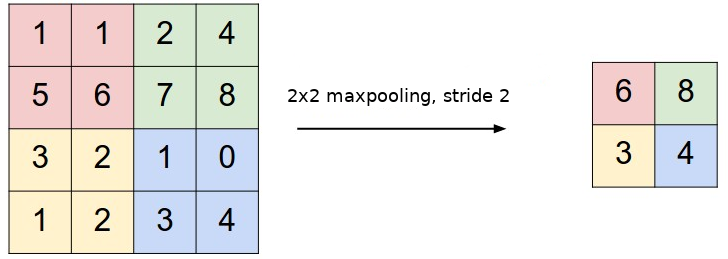
\includegraphics[scale=0.7]{maxpool.png}
  	\caption{Maxpooling med $k=2$ och $s=2$ av ett område med dimensioner $4 \times 4$ där resultatet bildar ett område med dimensionerna $2 \times 2$.}
\end{figure}

Liknande konvolutionslagret utan zero-padding blir det nästintillkommande lagrets dimensioner: \cite{cs231n} \cite{convmath} \cite{convarithmetic}
\begin{equation}
W' = \frac{W-k}{s}+1
\end{equation}
\begin{equation}
H' = \frac{H-k}{s}+1
\end{equation}
\begin{equation}
C' = C
\end{equation}
Antal kanaler förblir konstant.

Matematiskt beskrivs maxpoollagret genom: \cite{cs231n} \cite{convmath}
\begin{equation}\label{maxpool}
X^{(l+1)}_{r,c',h',w'} = \underset{0 \leq j < k, \ 0 \leq i < k}{\max} X^{(l)}_{r,c',(h's+j),(w's+i)}
\end{equation}
\subsubsection{Maxpoollagret bakåtpropagering}
Maxpooling saknar vikter och därmed är $\inpd{L(W)}{W^{(l)}}$ tom. Det som återstår är bakåtpropageringen av delta-felet. Med hjälp av kedjeregeln kan man dela upp derivatan i två bråk, $\inpd{L(W)}{X^{(l+1)}_{r,c',h',w'}}$ och $\inpd{X^{(l+1)}_{r,c',h',w'}}{X^{(l)}_{r,c,h,w}}$. $\inpd{L(W)}{X^{(l+1)}_{r,c',h',w'}}$ är den rekursiva delta-delet. $X^{(l+1)}_{r,c',h',w'}$ byts sedan ut mot dess definition enligt ekvation \eqref{maxpool}: \cite{cs231n} \cite{convmath} \cite{webconv3}

\begin{equation}
\begin{split}
	\delta^{(l)}_{r,c,h,w}
		& = \pd{L(W)}{X^{(l)}_{r,c,h,w}} \\
		& = \pd{L(W)}{X^{(l+1)}_{r,c',h',w'}} \pd{X^{(l+1)}_{r,c',h',w'}}{X^{(l)}_{r,c,h,w}} \\
		& = \delta_{r,c',h',w'} \pd{\underset{0 \leq j < k,0 \leq i < k}{\max} X^{(l)}_{r,c',(h's+j),(w's+i)}}{X^{(l)}_{r,c,h,w}} \\
\end{split}
\end{equation}
Den partiella derivatan i den sista ekvationen kommer vara lika med 1 om $X^{(l)}_{r,c',(h's+j),(w's+i)} = X^{(l)}_{r,c,h,w}$. I annat fall kommer $X^{(l)}_{r,c,h,w}$ inte ha någon påverkan på neuron index ${(r,c,h,w)}$ i lager $l+1$ och den partiella derivatan blir lika med 0: \cite{cs231n} \cite{convmath} \cite{webconv3}
\begin{equation}
\delta^{(l)}_{r,c,h,w} = \begin{cases}
				\delta_{r,c,h',w'} & \mbox{om } \begin{split} h = h's+j, \\w = w's+i \end{split}\\
				0 & \mbox{i annat fall}\\
			\end{cases}
\end{equation}

Alltså omdiregeras delta-felet till det ansvariga neuronet vars index kommer att behöva hållas i minnet. Om det finns två eller fler sektioner med samma neuron som är ansvarig för framåtpropageringen så kommer delta-felen summeras från samtliga korresponderande sektioners delta-fel. \cite{cs231n} \cite{convmath} \cite{webconv3}

\subsubsection{Batch Normalization framåtpropagering}
Utan Batch Normalization (BN) är det svårt att få djupa nätverk att divergera. Detta är till följd av att en liten ändring till det första lagret kan leda till en kaskad av förändringar i de senare lagren. I litteraturen kallas detta för \textit{internal covariate shift}. BN försöker att minimera denna \textit{internal covariate shift} genom att med avseende på alla exempel i mini-hopen normalisera varje feature map till varje lager. Resultatet är snabbare divergens och att det tillåter större träningshastigheter. Alltså har att man bearbetar flera exemepl i taget i en mini-hop en annan praktiska tillämpning än att försnabba uträkningar. \cite{cs231n} \cite{batchnorm}

Igen är aktiveringen vid lager $l$ och $l+1$ $X^{(l)} \in \mathbb{R}^{R \times C \times H \times W}$ respektive $X^{(l+1)} \in \mathbb{R}^{R \times C' \times H' \times W'}$. BN har ingen påverkan på dimensionerna av aktiveringen. \cite{cs231n} \cite{batchnorm}

Först beräknas medelvärdena $\mu_c$ och varianserna $\sigma^2_c$ till varje feature map $c$: \cite{cs231n} \cite{batchnorm}
\begin{equation}
\mu_c = \frac{1}{RHW} \sum^{R-1}_{r=0} \sum^{H-1}_{h=0} \sum^{W-1}_{w=0} X^{(l)}_{r,c,h,w}
\end{equation}
\begin{equation}
\sigma^2_c  = \frac{1}{RHW} \sum^{R-1}_{r=0} \sum^{H-1}_{h=0} \sum^{W-1}_{w=0} ({X^{(l)}_{r,c,h,w} - \mu_c})^2
\end{equation}
Sedan beräknas den normaliserade aktiveringen $\hat{X}$. Epsilon används för numerisk stabilitet. \cite{cs231n} \cite{batchnorm}
\begin{equation}
\hat{X}_{r,c,h,w} = (X^{(l)}_{r,c,h,w} - \mu_c){(\sigma^2_c + \epsilon)}^{-\frac{1}{2}}
\end{equation}
Sist introduceras 2 vikter, $\gamma_{c'}^{(l)}$ och $\beta_{c'}^{(l)}$, vilka tillåter nätverket att upphäva normaliseringen om nätverket dömmer det att vara användbart. \cite{cs231n} \cite{batchnorm}
\begin{equation}
X^{(l+1)}_{r,c,h,w} = \gamma_{c}^{(l)} \hat{X}_{r,c,h,w} + \beta_{c}^{(l)}
\end{equation}

Vid RUNTIME är det dock inte alltid möjligt att beräkna medelvärdet och variansen av mini-hopen på grund av att man oftast enbart vill testa ett exempel i taget. Medelvärdet och variansen för hela populationen måste då räknas ut och användas i stället för de beräknade värdena. Detta kan göras för små DATASETS, men om man arbetar med data som innehåller miljontals exempel är det enklare att uppskatta populationens statistik med hjälp av att updatera ett exponensiellt glidande medelvärde (EWMA) vid varje framåtpropagering: \cite{cs231n} \cite{batchnorm}
\begin{equation}
\mu_{EWMA_c} \to \lambda \mu_c + (1-\lambda)\mu_{EWMA_c}
\end{equation}
\begin{equation}
\sigma^2_{EWMA_c} \to \lambda \sigma^2_c + (1-\lambda)\sigma^2_{EWMA_c}
\end{equation}

Där $\mu_{EWMA_c}$ och $\sigma^2_{EWMA_c}$ betäcknar de exponensiella glidande medelvärdena och $\lambda$ betäcknar dämpfaktorn.


\subsubsection{Batch Normalization bakåtpropagering}
För BN behöver det rekursiva delta-felet $\delta^{(l)}$, derivatan av kostandsfunktionen med avseende på $\gamma_{c'}^{(l)}$ och derivatan av kostandsfunktionen med avseende på $\beta{c'}^{(l)}$ beräknas. För att beräkna detta krävs något som heter kronecker-deltat, oftast betäcknat med $\delta_{i,j}$ men kommer vara betäcknat med $I_{i,j}$ i denna rapport på grund av $\delta$ används för en annan term. Kronecker-deltat har följande egenskaper: \cite{webBN1} \cite{webBN2}
\begin{equation}\label{kroneckerdelta}
I_{i,j} = \begin{cases} 1 & \mbox{om } i = j \\ 0 & \mbox{om } i \neq j  \end{cases}
\end{equation}
\begin{equation}\label{kroneckerdeltaDERIVATIVE}
\pd{a_{j}}{a_i} = I_{i,j}
\end{equation}
\begin{equation}\label{kroneckerdeltaSUM}
\sum_j  a_i  I_{i,j} = a_j
\end{equation}
Först bryts $\inpd{L(W)}{X^{(l)}}$ upp i tre bråk och sedan summeras alla partiella derivator likt ekvation \eqref{konvolutionbackprop}. \cite{webBN1} \cite{webBN2} Här summeras dessutom R-dimensionen på grund av att aktiveringar från hela mini-hopen har en påverkan på $\delta^{(l)}$.
\begin{align}\label{BN_delta_error}
\begin{split}
	\delta^{(l)}_{r,c,h,w}
		& = \pd{L(W)}{X^{(l)}_{r,c,h,w}} \\
		& = \sum^{R'-1}_{r'=0} \sum^{C'-1}_{c'=0} \sum^{H'-1}_{h'=0} \sum^{W'-1}_{w'=0} \pd{L(W)}{X^{(l+1)}_{r',c',h',w'}} \pd{X^{(l+1)}_{r',c',h',w'}}{\hat{X}_{r',c',h',w'}} \pd{\hat{X}_{r',c',h',w'}}{{X}^{(l)}_{r,c,h,w}}\\
\end{split}
\end{align}

$\inpd{L(W)}{X^{(l+1)}_{r,c,h,w}}$ är det föregående rekursiva delta-felet. $\inpd{X^{(l+1)}_{r',c',h',w'}}{\hat{X}_{r',c',h',w'}}$ hittas enkelt på grund av att den är en linjär funktion. \cite{webBN1} \cite{webBN2}

\begin{equation}\label{BN_dxdxhat}
\begin{split}
	\pd{X^{(l+1)}_{r',c',h',w'}}{\hat{X}_{r',c',h',w'}}
		& = \pd{(\gamma_{c'}^{(l)} \hat{X}_{r',c',h',w'} + \beta_{c'}^{(l)})}{\hat{X}_{r',c',h',w'}} \\
		& =\gamma_{c'}^{(l)}
\end{split}
\end{equation}

För derivatan av den centrerade aktiveringen med avseende på den originella aktiveringen tillämpas produktregeln: \cite{webBN1} \cite{webBN2}
\begin{equation}\label{BN_kedjeregeln}
\begin{split}
\pd{\hat{X}_{r',c',h',w'}}{{X}^{(l)}_{r,c,h,w}} 
	& = \pd{(X^{(l)}_{r',c',h',w'} - \mu_{c'}){(\sigma^2_{c'} + \epsilon)}^{-\frac{1}{2}}}{{X}^{(l)}_{r,c,h,w}} \\
	& = {(\sigma^2_{c'} + \epsilon)}^{-\frac{1}{2}} \pd{(X^{(l)}_{r',c',h',w'} - \mu_{c'})}{{X}^{(l)}_{r,c,h,w}} - \frac{1}{2}(X^{(l)}_{r',c',h',w'} - \mu_c){(\sigma^2_{c'} + \epsilon)}^{-\frac{3}{2}} \pd{\sigma^2_{c'}}{{X}^{(l)}_{r,c,h,w}}
\end{split}
\end{equation}

Derivatan av den första faktorn med avseende på aktiveringen beräknas med hjälp av ekvationer \eqref{kroneckerdelta}, \eqref{kroneckerdeltaDERIVATIVE} och \eqref{kroneckerdeltaSUM}. \cite{webBN1} \cite{webBN2}
\begin{equation}\label{mu'}
\begin{split}
\pd{(X^{(l)}_{r',c',h',w'} - \mu_{c'})}{{X}^{(l)}_{r,c,h,w}}
	& = \pd{({X^{(l)}_{r',c',h',w'} - \frac{1}{RHW} \sum\limits^{R-1}_{r''=0} \sum\limits^{H-1}_{h''=0} \sum\limits^{W-1}_{w''=0} X^{(l)}_{r'',c',h'',w''}})}{{X}^{(l)}_{r,c,h,w}} \\
	& = I_{r',r} I_{c',c} I_{h',h} I_{w',w} - \frac{1}{RHW} I_{c',c}
\end{split}
\end{equation}

Derivatan av den andra faktorn med avseende på aktiveringen beräknas på ett liknande sätt med hjälp av kedjeregeln och ekvationer \eqref{kroneckerdelta}, \eqref{kroneckerdeltaDERIVATIVE} och \eqref{kroneckerdeltaSUM}. \cite{webBN1} \cite{webBN2}
\begin{equation}\label{sigma'}
\begin{split}
\pd{\sigma^2_{c'}}{{X}^{(l)}_{r,c,h,w}}
	& = \pd{\frac{1}{RHW} \sum\limits^{R-1}_{r'=0} \sum\limits^{H-1}_{h'=0} \sum\limits^{W-1}_{w'=0} ({X^{(l)}_{r',c',h',w'} - \mu_{c'}})^2}{{X}^{(l)}_{r,c,h,w}} \\
	& = \frac{1}{RHW} \sum\limits^{R-1}_{r'=0} \sum\limits^{H-1}_{h'=0} \sum\limits^{W-1}_{w'=0} 2 ({X^{(l)}_{r',c',h',w'} - \mu_{c'}}) (I_{r',r} I_{c',c} I_{h',h} I_{w',w} - \frac{1}{RHW} I_{c',c}) \\
	& = \frac{2}{RHW} ({X^{(l)}_{r,c',h,w} - \mu_{c'}})I_{c',c} - \frac{2}{(RHW)^2}  \sum\limits^{R-1}_{r'=0} \sum\limits^{H-1}_{h'=0} \sum\limits^{W-1}_{w'=0} ({X^{(l)}_{r',c,h',w'} - \mu_{c}}) \\
	& = \frac{2}{RHW} ({X^{(l)}_{r,c',h,w} - \mu_{c'}})I_{c',c}
\end{split}
\end{equation}
Den sista summan blir lika med noll på grund av att termerna summeras ihop till medelvärdet minus medelvärdet. 

När alla komponenter till bakåtpropageringen av delta-felet är beräknade är insättning av ekvation \eqref{BN_kedjeregeln}, \eqref{mu'} och \eqref{sigma'} i ekvation \eqref{BN_delta_error} det enda som kvarstår:

\begin{multline}
	\delta^{(l)}_{r,c,h,w} = \sum^{R'-1}_{r'=0} \sum^{C'-1}_{c'=0} \sum^{H'-1}_{h'=0} \sum^{W'-1}_{w'=0} \pd{L(W)}{X^{(l+1)}_{r',c',h',w'}} \pd{X^{(l+1)}_{r',c',h',w'}}{\hat{X}_{r',c',h',w'}} \pd{\hat{X}_{r',c',h',w'}}{{X}^{(l)}_{r,c,h,w}}\\
		\qquad = \sum\limits_{r',c',h',w'}\delta^{(l+1)}_{r',c',h',w'} \gamma^{(l)}_{c'} {(\sigma^2_{c'} + \epsilon)}^{-\frac{1}{2}} (I_{r',r} I_{c',c} I_{h',h} I_{w',w} - \frac{1}{RHW} I_{c',c}) \\
	-\sum\limits_{r',c',h',w'}\delta^{(l+1)}_{r',c',h',w'} \gamma^{(l)}_{c'} \frac{1}{RHW} ({X^{(l)}_{r',c',h',w'} - \mu_{c'}})({X^{(l)}_{r,c',h,w} - \mu_{c'}}) {(\sigma^2_{c'} + \epsilon)}^{-\frac{3}{2}} I_{c',c} \\
	\quad = \delta^{(l+1)}_{r,c,h,w} \gamma^{(l)}_{c} {(\sigma^2_{c} + \epsilon)}^{-\frac{1}{2}} - \frac{1}{RHW} \sum\limits_{r',h',w'} \delta^{(l+1)}_{r',c,h',w'} \gamma^{(l)}_{c} {(\sigma^2_{c} + \epsilon)}^{-\frac{1}{2}}\\
	- \frac{1}{RHW} \sum\limits_{r',h',w'} \delta^{(l+1)}_{r',c,h',w'}\gamma^{(l)}_{c} ({X^{(l)}_{r',c,h',w'} - \mu_{c'}})({X^{(l)}_{r,c,h,w} - \mu_{c}}){(\sigma^2_{c} + \epsilon)}^{-\frac{3}{2}} \\
	= \frac{1}{RHW} \gamma^{(l)}_c {(\sigma^2_{c} + \epsilon)}^{-\frac{1}{2}} \biggl(    RHW \delta^{(l+1)}_{r,c,h,w} -  \sum\limits_{r',h',w'} \delta^{(l+1)}_{r',c,h',w'} \qquad \\
	-  ({X^{(l)}_{r,c,h,w} - \mu_{c}}) {(\sigma^2_{c} + \epsilon)}^{-\frac{3}{2}} \sum\limits_{r',h',w'} \delta^{(l+1)}_{r',c,h',w'} ({X^{(l)}_{r',c,h',w'} - \mu_{c'}}) \biggl) \\
\end{multline}

Derivatan av vikterna hittas på ett liknande sätt med en faktor $\frac{1}{R}$ på grund av att det är medelvärdet för alla exemepl i mini-hopen som är eftersökt. \cite{webBN1} \cite{webBN2}
\begin{align}
\begin{split}
	\pd{L(W)}{\gamma^{(l)}_{c}}
		& = \frac{1}{R}\sum^{R-1}_{r} \sum^{C'-1}_{c'} \sum^{H'-1}_{h'} \sum^{W'-1}_{w'} \pd{L(W)}{X^{(l+1)}_{r,c',h',w'}} \pd{X^{(l+1)}_{r,c',h',w'}}{\gamma^{(l)}_{c}} \\
		& = \frac{1}{R}\sum^{R-1}_{r} \sum^{C'-1}_{c'} \sum^{H'-1}_{h'} \sum^{W'-1}_{w'} \delta^{(l+1)}_{r,c',h',w'}  \pd{({\gamma_{c'}^{(l)} \hat{X}_{r,c',h',w'} + \beta_{c'}^{(l)}})}{\gamma^{(l)}_{c}} \\
		& = \frac{1}{R}\sum^{R-1}_{r} \sum^{C'-1}_{c'} \sum^{H'-1}_{h'} \sum^{W'-1}_{w'} \delta^{(l+1)}_{r,c',h',w'} \hat{X}_{r,c,h',w'} I_{c',c}\\
		& = \frac{1}{R}\sum^{R-1}_{r} \sum^{H'-1}_{h'} \sum^{W'-1}_{w'} \delta^{(l+1)}_{r,c,h',w'} \hat{X}_{r,c,h',w'} \\
\end{split}
\end{align}


\begin{align}
\begin{split}
	\pd{L(W)}{\beta^{(l)}_{c}}
		& = \frac{1}{R}\sum^{R-1}_{r} \sum^{C'-1}_{c'} \sum^{H'-1}_{h'} \sum^{W'-1}_{w'} \pd{L(W)}{X^{(l+1)}_{r,c',h',w'}} \pd{X^{(l+1)}_{r,c',h',w'}}{\beta^{(l)}_{c}} \\
		& = \frac{1}{R}\sum^{R-1}_{r} \sum^{C'-1}_{c'} \sum^{H'-1}_{h'} \sum^{W'-1}_{w'} \delta^{(l+1)}_{r,c',h',w'}  \pd{({\gamma_{c'}^{(l)} \hat{X}_{r,c',h',w'} + \beta_{c'}^{(l)}})}{\beta^{(l)}_{c}} \\
		& = \frac{1}{R}\sum^{R-1}_{r} \sum^{C'-1}_{c'} \sum^{H'-1}_{h'} \sum^{W'-1}_{w'} \delta^{(l+1)}_{r,c,h',w'} I_{c',c}\\
		& = \frac{1}{R}\sum^{R-1}_{r} \sum^{H'-1}_{h'} \sum^{W'-1}_{w'} \delta^{(l+1)}_{r,c,h',w'} \\
\end{split}
\end{align}

\subsection{Praktiska Tillämpningar}
All kod till de exempel på praktiska tillämpningar kan hittas på github: \url{https://github.com/nikitazozoulenko}
\subsubsection{Klassificering av handskrivna siffror}
En enkel CNN-modell kan användas för att klassificera handskriva siffror. För att uppnå detta har MNIST DATASET för handskriva siffror används. Den består av 60 000 unika exempel för träning och ytterligare 10 000 exempel för validering av modellen. Valideringsdatan måste vara separerad från datan man tränar med för annars finns det risk att modellen OVERFITTAS och inte kan generalisera för andra exempel än träningsdatan. \cite{MNIST}

Låt modellens prognos betäcknas med $\hat{y}$. Aktiveringsfunktionen softmax används i det sista lagret för att gränsa värdena till intervallet $[0,1]$ och har egenskapen att alla prognostiserade värdena i ett exempel summeras till 1. Följaktligen kan varje värde i $\hat{y}$ tolkas som sannolikheten att bilden är av varje klass. \cite{cs231n}

\begin{figure}[h]\label{figMNIST}
	\centering
  		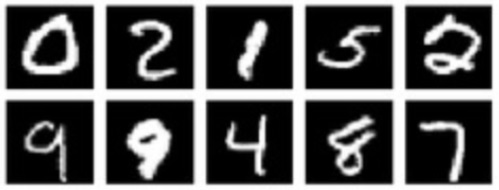
\includegraphics[scale=1]{mnist.png}
  	\caption{Tio bilder av handskrivna siffror från MNIST DATASETET. \cite{MNIST}}
\end{figure}

Input för modellen är en $28 \times 28$ pixelarray. Modellen prognostiserar tio värden per bild i form av en tensor $\hat{y} \in \mathbb{R}^{R \times C}$, ett värde för varje klass $C=10$ av siffra. Om det näst sista lagret är $x$ med samma dimensioner som $\hat{y}$ definieras softmaxfunktionen $P$ genom: \cite{cs231n} \cite{notesonbackprop} \cite{websoftmax} 
\begin{equation}
\begin{split}
P(x_{r,c}) 
	& = \hat{y}_{r,c} \\
	& = \dfrac{e^{x_{r,c}}}{\sum^{C-1}_{c'=0}e^{x_{r,c'}}}\\
\end{split}
\end{equation}

\begin{equation}
\begin{split}
\pd{P(x_{r,c})}{x_{r,c''}}
	& = \dfrac{(\sum^{C-1}_{c'=0}e^{x_{r,c'}}) (e^{x_{r,c}})I_{c,c''} - (e^{x_{r,c}})(\sum^{C-1}_{c'=0}e^{x_{r,c'}} I_{c',c''})}{(\sum^{C-1}_{c'=0}e^{x_{r,c'}})^2} \\
	& = \dfrac{(e^{x_{r,c}})I_{c,c''}}{\sum^{C-1}_{c'=0}e^{x_{r,c'}}} - \dfrac{(e^{x_{r,c}})(e^{x_{r,c''}})}{(\sum^{C-1}_{c'=0}e^{x_{r,c'}})^2} \\
	& = \hat{y}_{r,c}(I_{c,c''}-\hat{y}_{r,c''})
\end{split}
\end{equation}
Där $I$ är kronecker-deltat.

Tillsammans med softmax används kostnadsfunktionen \textit{cross entropy} betäcknat med $L$ där $y$ är THE GROUND TRUTH: \cite{cs231n} \cite{notesonbackprop}

\begin{equation}
L(W) = - \frac{1}{R}\sum^{R-1}_{r=0} \sum^{C-1}_{c=0}y_{r,c} \ \log{\hat{y}_{r,c}}
\end{equation}
\begin{equation}
\begin{split}
\pd{L(W)}{\hat{y}_{r',c'}} 
	& = \pd{\left(-\frac{1}{R}\sum^{R-1}_{r=0} \sum^{C-1}_{c=0}y_{r,c} \ \log{\hat{y}_{r,c}}\right)}{\hat{y}_{r',c'}} \\
	& = -\frac{1}{R}\sum^{R-1}_{r=0} \sum^{C-1}_{c=0}y_{r,c} \pd{\left(\log{\hat{y}_{r,c}}\right)}{\hat{y}_{r',c'}} \\
	& = - \frac{1}{R}\sum^{R-1}_{r=0} \sum^{C-1}_{c=0} y_{r,c} \frac{1}{\hat{y}_{r,c}} I_{r, r'} I_{c, c'}\\
	& = - \frac{1}{R} \frac{y_{r',c'}}{\hat{y}_{r',c'}} \\
\end{split}
\end{equation}

Där $I$ är kronecker-deltat.

Endast två olika modeller med olika lagerstrukturer prövades på grund av begränsad datakraft. En hopstorlek av 50 användes och 1200 iterationer av framåt- och bakåtpropagering kördes på den egenimplementerade modellen skriven i python. Totalt tog det 50 minuter för varje modell.

\begin{center}
    \begin{tabular}{ | c |}
    \hline
    		\textbf{Modell 1} \\ \hline \hline
    		Input \\ \hline
    		BN \\ \hline
            conv3 c16 s1\\ \hline
            maxpool2 s2\\ \hline
            ReLU\\ \hline
            BN\\ \hline
            conv3 c16 s1\\ \hline
            ReLU\\ \hline
            BN\\ \hline
            conv4 c16 s1\\ \hline
            maxpool2 s2\\ \hline
            ReLU\\ \hline
            BN\\ \hline
            conv4 c10 s1\\ \hline
            softmax \\ \hline
            Output \\
    \hline
    \end{tabular}
	\qquad   
    \begin{tabular}{ | c |}
    \hline
    		\textbf{Modell 2} \\ \hline \hline
 			Input \\ \hline
 			BN \\ \hline
            conv3 c16 s1 \\ \hline
            ReLU \\ \hline
            BN \\ \hline
            conv3 c16 s1\\ \hline
            ReLU\\ \hline
            BN\\ \hline
            conv3 c16 s1\\ \hline
            maxpool2 s2\\ \hline
            ReLU\\ \hline
            BN\\ \hline
            conv4 c16 s1\\ \hline
            ReLU\\ \hline
            BN\\ \hline
            conv4 c24 s1\\ \hline
            ReLU\\ \hline
            BN\\ \hline
            conv3 c24 s1\\ \hline
            ReLU\\ \hline
            BN\\ \hline
            conv3 c10 s1\\ \hline
            softmax \\ \hline
            Output \\
    \hline
    \end{tabular}
\end{center}

Ett lager är antingen BN, conv (konvolution), maxpool, softmax eller ReLU. Nästinkommande siffra efter lagernamnet är kärnstorleken. $C$ benämner antal kärner vid det lagret och därmed antal kanaler vid nästa lager. Klivet benämns med $s$.

Modell 1 uppnådde $95.57\%$ precision medan modell 2 uppnådde $98.07\%$ precision. Efter testerna kördes tränades det bättre presternade nätverket, modell 2, på fler iterationer tills validationsprecisionen började avta. Den testades varje 60 000 exemepel eller efter varje 600 iterationer med en hopstorlek av 100. Efter varje 60 000 bilder blandades dem för att förbättra inlärningen.

\begin{figure}[h]\label{figkosnadmnist}
	\centering
  		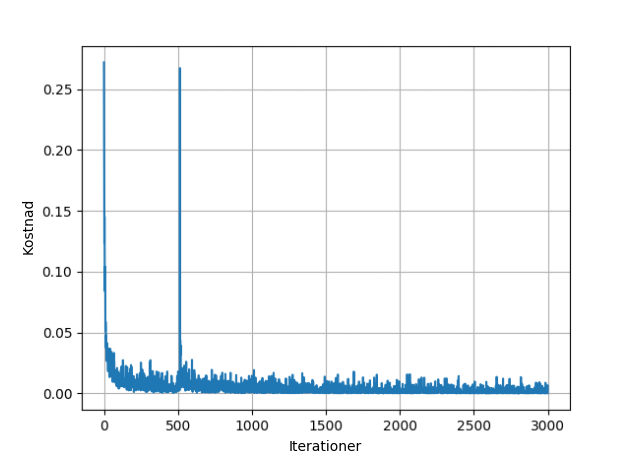
\includegraphics[scale=0.6]{kostandsplot.png}
  	\caption{En graf av kostnadsfunktionen efter varje iteration av mini-hopen av 100 bilder.}
\end{figure}
\begin{figure}[h]\label{figepokmnist}
	\centering
  		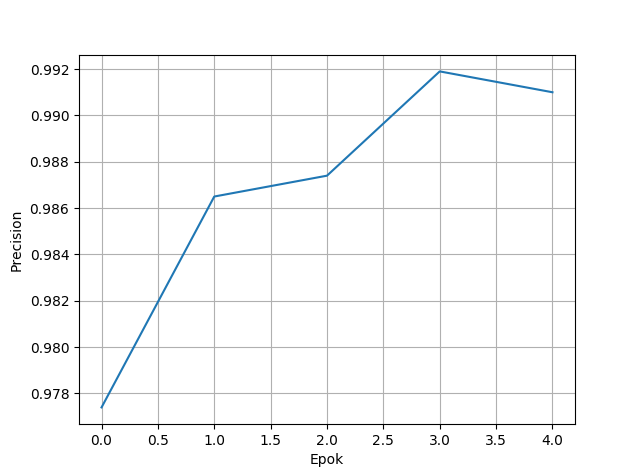
\includegraphics[scale=0.6]{epokplot.png}
  	\caption{En graf av validationsprecisionen efter varje epok av 60 000 bilder med modell 2.}
\end{figure}

Den slutgiltiga precisionen blev $99.2\%$. Av 10 000 handskrivna siffror lyckades modellen klassifisera 9 919 siffror rätt.

\subsubsection{Objektdetektering i bilder}
Om modellen YOLO:

\subsubsection{Ansiktsigenkänning}
anpassar yolo till en ansiktsdatabas

\section{Diskussion}
Vet inte vad jag ska diskutera?????

Matten går inte att argumentera med. Det som skulle kunna pratas om är hur jag skulle kunna förbättra modellerna, med det är ju ganska jävla svårt för det här är state of the art. Jag förstår inte det som folk gör för att förbättra det jag har gjort.



\begin{thebibliography}{99}
%%  Start of bibliography. It works almost exactly like a list, but with 
%%  \bibitem instead of \item. 
%%    
    

	
\bibitem{cs231n} 
	\textit{CS231n: Convolutional Neural Networks for Visual Recognition.}
    F. Li, A. Karpathy och J. Johnson.
	Stanford University, föreläsning, vinter 2016.
	
\bibitem{notesonbackprop} 
	\textit{Notes on Backpropagation.}
    P. Sadowski.
    University of California Irvine	Department of Computer Science.
    
\bibitem{convmath} 
	\textit{Introduction to Convolutional Neural Networks.}
    J. Wu. 
    National Key Lab for Novel Software Technology, Nanjing University, Kina.
    1 maj, 2017.

\bibitem{convarithmetic} 
	\textit{A guide to convolution arithmetic for deep learning.}
    V. Dumoulin  och F. Visin.
    FMILA, Université de Montréal. AIRLab, Politecnico di Milano.
	24 mars, 2016.

\bibitem{highperformanceconv} 
	\textit{High Performance Convolutional Neural Networks for Document Processing.}
    K. Chellapilla, S. Puri, P. Simard.
    Tenth International Workshop on Frontiers in Handwriting Recognition. 
    La Baule, Frankrike, Suvisoft.
	Oktober 2006.

\bibitem{wikiStanford} 
	\textit{Unsupervised Feature Learning and Deep Learning.}
    Standford University, Department of Computer Science.
    URL http://ufldl.stanford.edu/wiki/.
	Senast uppdaterad 31 mars 2013.
	
\bibitem{gradient} 
	\textit{Scientific Computing 2013, Worksheet 6: Optimization: Gradient and steepest descent.}
    University of Tartu, Estland.
    2013.
    
\bibitem{yolo} 
	\textit{You only look once: Unified, real-time object detection.}
    J. Redmon, S. Divvala, R. Girshick, och A. Farhadi. 
    arXiv preprint arXiv:1506.02640, 2015.

\bibitem{resnet} 
	\textit{Deep residual learning for image recognition.}
    K. He, X. Zhang, S. Ren, och J. Sun. 
    arXiv preprint arXiv:1512.03385, 2015.
    
\bibitem{batchnorm} 
	\textit{Batch normalization: Accelerating deep network training by reducing internal covariate shift.}
    S. Ioffe och C. Szegedy. 
	arXiv preprint arXiv:1502.03167, 2015.
    
\bibitem{webconv1} 
	\textit{Backpropagation In Convolutional Neural Networks.}
	J. Kafunah.
    DeepGrid, Organic Deep Learning. 
    URL http://www.jefkine.com/.
	5 september 2016.

\bibitem{webBN1} 
	\textit{What does the gradient flowing through batch normalization looks like?}
	C. Thorey.
    Machine Learning Blog. 
    URL http://cthorey.github.io/.
	28 januari 2016.
	
\bibitem{webconv2} 
	\textit{Note on the implementation of a convolutional neural networks.}
	C. Thorey.
    Machine Learning Blog. 
    URL http://cthorey.github.io/.
	2 februari 2016.
	
\bibitem{webBN2} 
	\textit{Understanding the backward pass through Batch Normalization Layer.}
	Flaire of Machine Learning
    URL https://kratzert.github.io.
	5 september 2016.
	
\bibitem{webconv3} 
	\textit{Convolutional Neural Networks.}
	A. Gibiansky.
    URL http://andrew.gibiansky.com.
	24 februari 2014.
	
\bibitem{websoftmax} 
	\textit{Classification and Loss Evaluation - Softmax and Cross Entropy Loss.}
	P. Dahal. 
	DeepNotes.
    URL https://deepnotes.io/softmax-crossentropy.
	24 februari 2014.
	
\bibitem{MNIST}
	\textit{The MNIST database of handwritten digits}
	Y. LeCun, C. Cortes och C. Burges. Courant Institute, NYU. Google Labs, New York. Microsoft Research, Redmond. 
	URL http://yann.lecun.com/exdb/mnist/.
	Hämtad 3 november 2017.
	
\bibitem{figSGD}
	\textit{Pygradsc.}
	J. Komoroske.
	URL https://github.com/joshdk/pygradesc.
	12 oktober 2012.
	
\bibitem{figboatcnn}
	\textit{Understanding Convolutional Neural Networks for NLP.}
	D. Britz.
	WildML, Artificial Intelligence, Deep Learning, and NLP.
	7 november 2015.
	
\bibitem{figkonv}
	\textit{Understanding Convolutional Neural Networks for NLP.}
	D. Britz.
	WildML, Artificial Intelligence, Deep Learning, and NLP.
	7 november 2015.
	
\bibitem{figconv}
	\textit{Deep learning for complete beginners: convolutional neural networks with keras.}
	P. Veličković.
	Camebridge Spark. 
	URL https://cambridgespark.com/content.
	Senast uppdaterad 20 mars 2017.
\end{thebibliography}


\end{document}